\documentclass[]{article}
\usepackage{amssymb}
\usepackage[backend=bibtex,style=authoryear,natbib=true]{biblatex} % Use the bibtex backend with the authoryear citation style (which resembles APA)

\addbibresource{example.bib} % The filename of the bibliography

\usepackage[autostyle=true]{csquotes} % Required to generate language-dependent quotes in the bibliography

\usepackage{tikz}
\usepackage{tikz-network}
\usepackage{breqn}

\usepackage{graphicx}
\usepackage{subcaption}
\usepackage{multirow}
\usetikzlibrary{fit}
\usetikzlibrary {arrows.meta,graphs,shapes.misc}
\usetikzlibrary {positioning}

\newcommand{\bn}{\textbf{n}}
\newcommand{\tabhead}[1]{\textbf{#1}}

\begin{document}

\section{Guided Gated Convolution Neural Network for Normal Inference }

The inference result of guided-GCNN model is shown in Figure \ref{fig:ng-eval-synthetic}. With adding the information of a gray-scale image, the model is able to sharpen the details over the whole scene. 

\begin{figure}[h!]
	\centering
	\begin{subfigure}[b]{0.19\linewidth}
		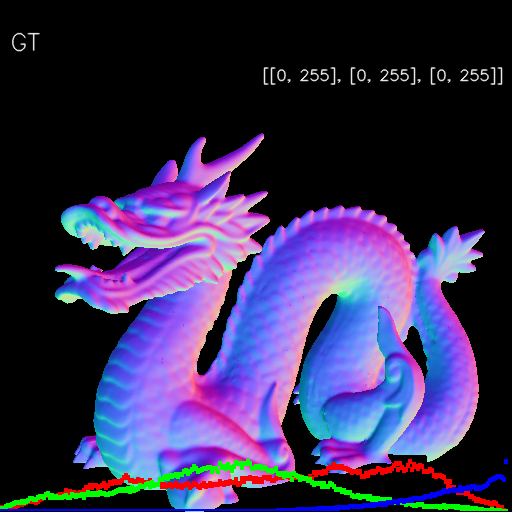
\includegraphics[width=\linewidth]{./Figures/ng-synthetic/fancy_eval_3_groundtruth.png}
		\caption{GT}
	\end{subfigure}
	\begin{subfigure}[b]{0.19\linewidth}
		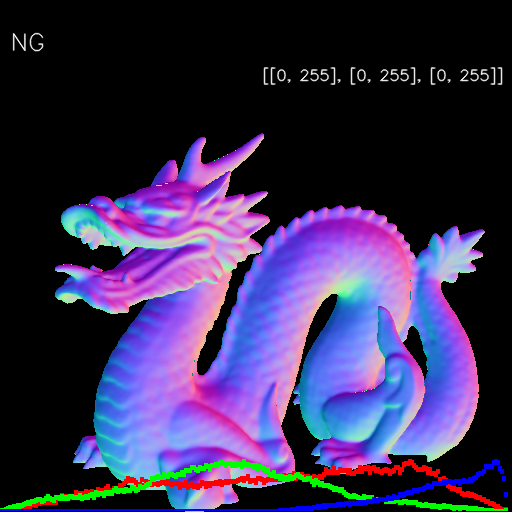
\includegraphics[width=\linewidth]{./Figures/ng-synthetic/fancy_eval_3_normal_NG.png}
		\caption{g-GCNN}
	\end{subfigure}
	\begin{subfigure}[b]{0.19\linewidth}
		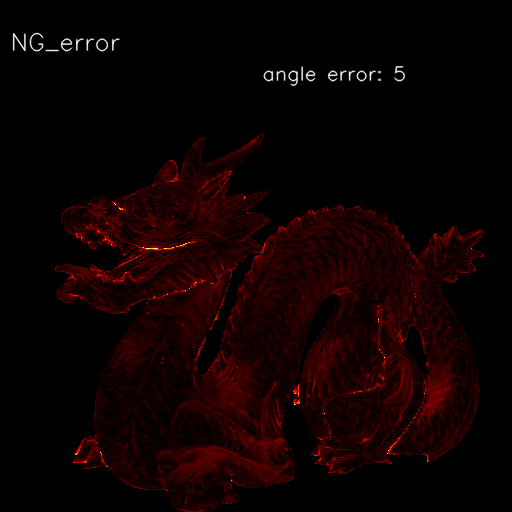
\includegraphics[width=\linewidth]{./Figures/ng-synthetic/fancy_eval_3_error_NG.png}
		\caption{Angle Error}
	\end{subfigure}
	\begin{subfigure}[b]{0.19\linewidth}
		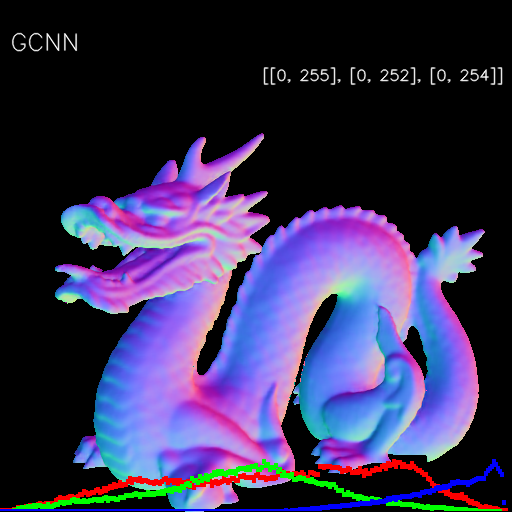
\includegraphics[width=\linewidth]{./Figures/gcnn-synthetic/fancy_eval_3_normal_GCNN.png}
		\caption{GCNN}
	\end{subfigure}
	\begin{subfigure}[b]{0.19\linewidth}
		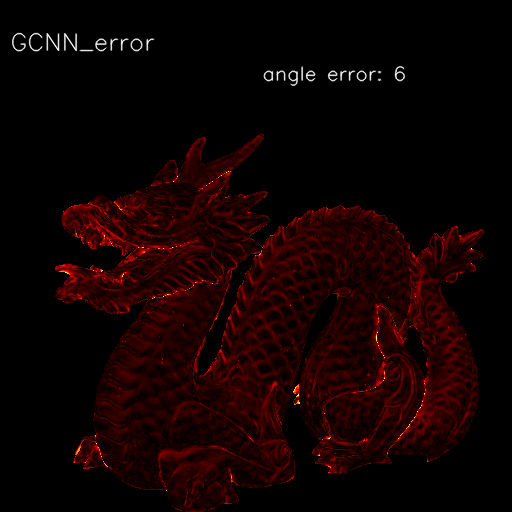
\includegraphics[width=\linewidth]{./Figures/gcnn-synthetic/fancy_eval_3_error_GCNN.png}
		\caption{Angle Error}
	\end{subfigure}
	\caption{guided-GCNN Normal Inference on Synthetic Dataset (object: dragon). GCNN result is shown on (d) and (e) as comparison.}
	\label{fig:ng-eval-synthetic}
\end{figure}




\end{document}
